\chapter{Charge transfer in amorphous systems}
\label{chap:surface_hopping_app}
Although it is important to know the maximum bound on the mobility of the charge carrier in a perfect crystal of an organic semiconductor, in reality it is very difficult to control defect formation in OSs\cite{NGUYEN2006198i, Ray2014}. This is due to van der Waals forces only weakly holding molecules at lattice sites, allowing molecules greater freedom than in traditional inorganic crystal, and increasing the chance of defect formation which can trap/scatter charge carriers reducing overall mobility. This means it is important to investigate and characterise charge transport properties for not just perfectly crystalline OSs but also those that show a range of amorphicity.
\\
\begin{wrapfigure}{r}{0.4\textwidth}
	\vspace*{-0.5cm}
	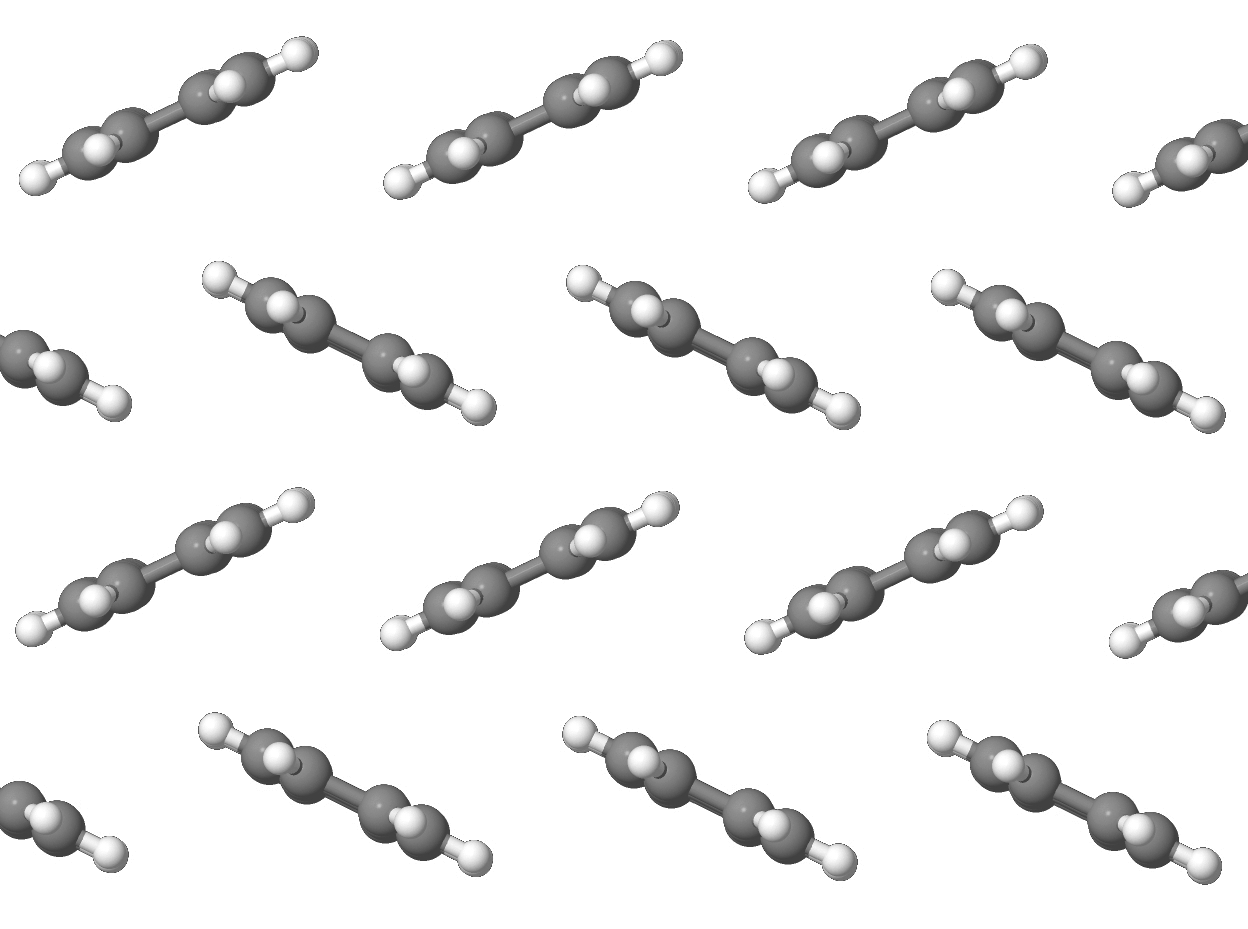
\includegraphics[width=0.4\textwidth]{img/herringbone.png}
	\caption{An example of the \\herringbone packing \\typically found in \\Pentacene crystals}
	\label{fig:HerringbonePacking}
\end{wrapfigure}
The molecule chosen to investigate amorphous films was pentacene. This molecule is a popular organic semiconductor and the subject of much research due to its high field effect mobility \cite{Hu2005}, use in device applications \cite{Hasegawa_2009} and, more recently, the use of functionalization to alter device properties \cite{Anthony2001, Anthony2002}. The pentacene molecule consists of 5 joined benzene rings (36 atoms) and crystals typically pack with a herringbone motif as shown in figure \ref{fig:HerringbonePacking}.
\section{Creating Amorphous Pentacene}
In order to create the amorphous pentacene systems a melt-quench technique was used...
